\subsection{Pick's Theorem}
\label{sec:pick}

Pick's Theorem gives a formula for the area of a polygon
in the plane with vertices on the lattice $\ZZ^2$ \cite{og-pick}.
We give a proof originally due to Blatter \cite{blatter_another_1997}
and restated by Tabachnikov  \cite{tabachnikov_proofs_2014}.

\begin{theorem}[Pick's Theorem]\label{thm:pick}
Let $P$ be a simple polygon in the plane with vertices on the lattice $\ZZ^2$,
let $I$ be the number of lattice points inside of $P$, let $B$ be the number
of lattice points on the boundary of $P$ and let $A$ denote the area of $P$.
Then, 
$$A=I+\frac{B}{2}-1.$$
\end{theorem}
See \figref{picks} for an example.

 \begin{figure}[htb]
         \centering
         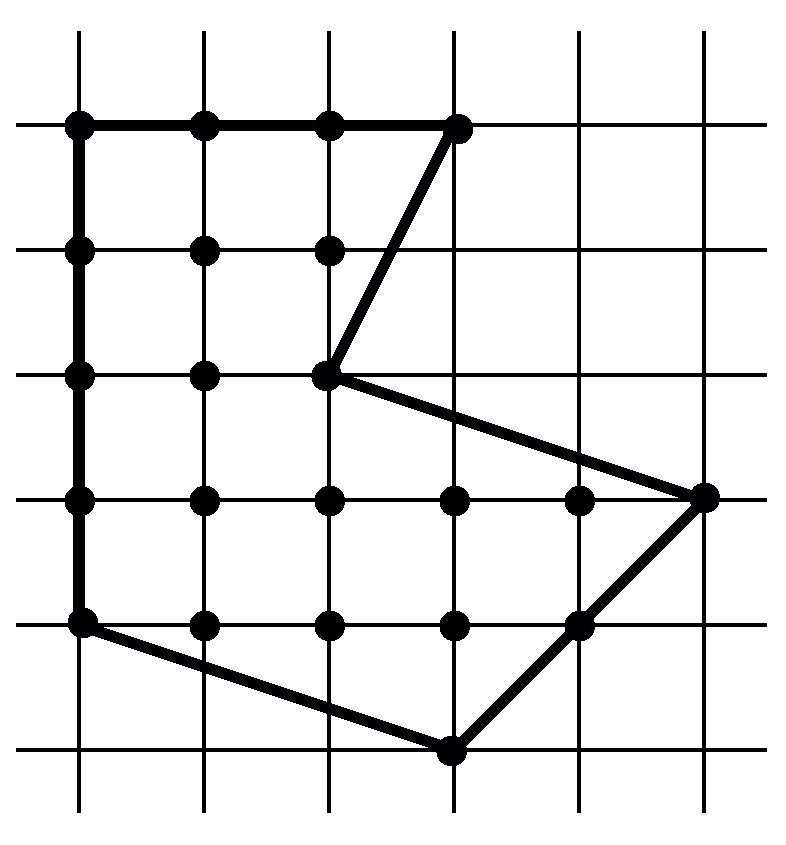
\includegraphics[width=5cm]{pick}
	\caption{A polygon with vertices on the lattice. 
	There are 10 interior vertices and 12 vertices on the boundary.
	By Pick's theorem the area of the polygon is $10+\frac{12}{2}-1=15.$
	\label{fig:picks}}
 \end{figure}
 
\begin{proof}
	Put a unit volume ice cube at each lattice point in the plane and let the ice melt.
	The water will evenly cover the plane with the amount of water inside the polygon 
	equal to its area.
	
	Consider a edge on the the polygon. The amount of water that flows
	into to polygon across this edge equals that amount of water that flows out of the polygon
	across this edge by symmetry. This is because the edge connects two lattice points,
	for each point the contributes flow across the edge in one direction there is a symmetric
	point that contributes and equal amount of flow in the opposite direction.
	So, the total flow across each edge is zero and
	the  amount of water inside the polygon comes from interior cubes and the lattice vertices
	of the polygon.
	
	Each interior lattice point contributes one unit of water. 
	Each lattice point on an edge, half of the water flows into the polygon and
	half flows outside of the polygon.
	Let $\alpha_i$ denote the interior angles at each vertex.
	Each vertex contributes $\frac{\alpha_i}{2\pi}$ units of water to the area.
	By the Gauss-Bonnet theorem, \thmref{simple-bonnet}, the sum of the interior
	angles is $\pi(n-2)$. Thus, the vertex points contribute a total of 
	$$\frac{\pi(n-2)}{2\pi}=\frac{n}{2}-1.$$
	The theorem follows.

\end{proof}

